\documentclass[12pt]{article}
\usepackage[utf8]{inputenc}

\usepackage{lmodern}

\usepackage{enumitem}
\usepackage[margin=2cm]{geometry}

\usepackage{amsmath, amsfonts, amssymb}
\usepackage{graphicx}
%\usepackage{subfigure}
\usepackage{tikz}
\usepackage{pgfplots}
\usepackage{multicol}

\usepackage{comment}
\usepackage{url}
\usepackage{calc}
\usepackage{subcaption}
\usepackage[indent=0pt]{parskip}
\usepackage{animate}

\usepackage{array}
\usepackage{blkarray,booktabs, bigstrut}
\usepackage{bigints}

\pgfplotsset{compat=1.16}

% MATH commands
\newcommand{\ga}{\left\langle}
\newcommand{\da}{\right\rangle}
\newcommand{\oa}{\left\lbrace}
\newcommand{\fa}{\right\rbrace}
\newcommand{\oc}{\left[}
\newcommand{\fc}{\right]}
\newcommand{\op}{\left(}
\newcommand{\fp}{\right)}

\newcommand{\bi}{\mathbf{i}}
\newcommand{\bj}{\mathbf{j}}
\newcommand{\bk}{\mathbf{k}}
\newcommand{\bF}{\mathbf{F}}

\newcommand{\mR}{\mathbb{R}}

\newcommand{\ra}{\rightarrow}
\newcommand{\Ra}{\Rightarrow}

\newcommand{\sech}{\mathrm{sech}\,}
\newcommand{\csch}{\mathrm{csch}\,}
\newcommand{\curl}{\mathrm{curl}\,}
\newcommand{\dive}{\mathrm{div}\,}

\newcommand{\ve}{\varepsilon}
\newcommand{\spc}{\vspace*{0.5cm}}

\DeclareMathOperator{\Ran}{Ran}
\DeclareMathOperator{\Dom}{Dom}

\newcommand{\exo}[1]{\noindent\textcolor{red}{\fbox{\textbf{Problem {#1}}}\hrulefill}\\}
\newcommand{\qu}[4]{\noindent\textcolor{#4}{\fbox{\textbf{Section {#1} | Problem {#2}}} \hrulefill{{\fbox{\textbf{{#3} Points}}}}\\}}

\newcommand{\semester}{Spring 2023}

\newcommand{\CVup}{%

\begin{tikzpicture}
\draw[black, <->, >=latex] (-0.33, 0.5) .. controls (-0.125, 0) and (0.125, 0) .. (0.33, 0.5);
\end{tikzpicture}}

\newcommand{\CVupInc}{%
\begin{tikzpicture}
\draw[black, ->, >=latex] (0,0) .. controls (0.2, 0) and (0.4, 0.2) .. (0.5, 0.5);
\end{tikzpicture}}

\newcommand{\CVupDec}{%
\begin{tikzpicture}[rotate=270]
\draw[black, ->, >=latex] (0,0) .. controls (0.2, 0) and (0.4, 0.2) .. (0.5, 0.5);
\end{tikzpicture}}

\newcommand{\CVdown}{%
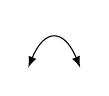
\begin{tikzpicture}
\draw[black, <->, >=latex] (-0.33, -0.5) .. controls (-0.125, 0) and (0.125, 0) .. (0.33, -0.5);
\end{tikzpicture}}

\newcommand{\CVdownInc}{%
\begin{tikzpicture}
\draw[black, ->, >=latex] (-0.5, -0.5) .. controls (-0.5, -0.3) and (-0.5, -0.1) .. (0,0);
\end{tikzpicture}}

\newcommand{\CVdownDec}{%
\begin{tikzpicture}[rotate=-90]
\draw[black, ->, >=latex] (-0.5, -0.5) .. controls (-0.5, -0.3) and (-0.5, -0.1) .. (0,0);
\end{tikzpicture}}

\begin{document}
	\noindent \hrulefill \\
	MATH-241 \hfill Pierre-Olivier Paris{\'e}\\
	Solutions Section 2-8 \hfill \semester \\\vspace*{-1cm}
	
	\noindent\hrulefill
	
	\spc
	
	\exo{6}
	\\
	We denote by
		\begin{itemize}
		\item $V(t)$: volume of the sphere (in $\textrm{mm}^3$).
		\item $r(t)$: radius of the sphere (in $\textrm{mm}$).
		\item $t$: time in seconds.
		\end{itemize}
	
	We know that
		\begin{align*}
		\frac{dr}{dt} = 4\textrm{mm}/s .
		\end{align*}
	The goal is to find
		\begin{align*}
		\left. \frac{dV}{dt} \right|_{r = 40} .
		\end{align*}
		
	The connection between $V$ and $r$ is
		\begin{align*}
		V = \frac{4}{3} \pi r^3 .
		\end{align*}
	Taking the derivative, we obtain
		\begin{align*}
		\frac{dV}{dt} = 4 \pi r^2 \big( \frac{dr}{dt} \big).
		\end{align*}
	Therefore, replacing $r$ by $40$, we get
		\begin{align*}
		\frac{dV}{dt} = 4 \pi (40)^2 4 = 25600 \pi\,  \textrm{mm}^3 .
		\end{align*}
	
	\spc
	
	\exo{12}
	\\
	We differentiate with respect $t$ the equation in $x$ and $y$ to get
		\begin{align*}
		x'y + x y' = 0..
		\end{align*}
	Replacing $x$ by $4$, $y$ by $2$, and $y' = -3$, we then obtain $x' = 6 \text{ cm/s}$.
	
	\spc
	
	\exo{16}
	\\
	First, let's draw a picture and introduce some notations.
	\begin{figure}[ht]
	\centering
	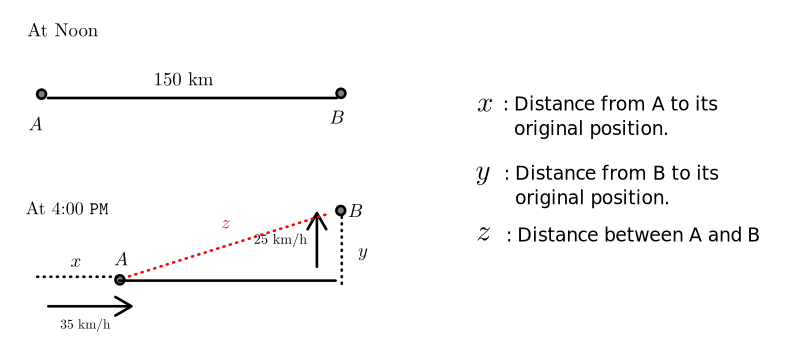
\includegraphics[scale=.65]{sec28-Prob16-illustration.png}
	\end{figure}
	The known information is $dx/dt = 35$ and $dy/dt = 25$. What we would like to know is $dz/dt$. 
	
	The link between $x$, $y$ and $z$ is given by the pythagorean Theorem:
		\begin{align*}
		z^2 = (150 - x)^2 + y^2
		\end{align*}
	where $150 - x$ is the distance from the boat $A$ to the original position of the boat $B$. Taking the derivative with respect to time gives
		\begin{align*}
		& \quad 2 z (dz/dt) = 2 (150 - x) (-dx/dt) + 2 y (dy/dt) . \\
		\iff & \quad dz/dt = ((150-x)/z) (-dx/dt) + (y/z) (dy/dt) .
		\end{align*}
	From noon to 4:00\textsc{pm}, the boat A travelled $4 \times 35 = 140 \text{ km}$ and the boat B travelled $4 \times 25 = 100 \text{ km}$. So $x = 140$, $y = 100$, and $z = \sqrt{10^2 + 100^2} = 10 \sqrt{101}$. Replacing everything in the last equations above, we obtain
		\begin{align*}
		dz/dt = (1/\sqrt{101}) (-35) + (10/\sqrt{101}) (25) = 215/\sqrt{101} \approx 25 \text{ km/h} .
		\end{align*}
	Thus, $dz/dt \approx 25 \text{ km/h}$.
	
	\spc
	
	\exo{22}
	\\
	We denote by
		\begin{itemize}
		\item $x(t)$: the distance from the bow of the boat and the bottom of the dock (in meters).
		\item $z(t)$: the distance from the bow of the boat and the dock.
		\item $t$: time in seconds.
		\end{itemize}
	
	We know that 
		\begin{align*}
		\frac{dz}{dt} = 1 \textrm{m}/\textrm{s} .
		\end{align*}
	The goal is to find
		\begin{align*}
		\left. \frac{dx}{dt} \right|_{x = 8m} .
		\end{align*}
		
	The connection between $z$ and $x$ is via the pythagorean theorem
		\begin{align*}
		x^2 + 1^2 = z^2 \quad \Ra \quad x^2 + 1 = z^2 .
		\end{align*}
	Taking the derivative, we find that
		\begin{align*}
		2x \frac{dx}{dt} = 2 z \frac{dz}{dt} \quad \Ra \quad x \frac{dx}{dt} = z \frac{dz}{dt} .
		\end{align*}
	With $x = 8$, we find that $z = \sqrt{1 + 8^2} = \sqrt{65}$. Therefore, pluging all the information in, we find
		\begin{align*}
		8 \frac{dx}{dt} = \sqrt{65} \cdot 1 \quad \Ra \quad \frac{dx}{dt} = \frac{\sqrt{65}}{8} \textrm{m}/\textrm{s} .
		\end{align*}
		
	
	
\end{document}